
\documentclass[a4paper,10pt]{beamer}
\usepackage[T1,plmath]{polski}
\usepackage[cp1250]{inputenc}
\usepackage{amssymb}
\usepackage{indentfirst}
\usepackage{graphicx}

\usefonttheme[onlymath]{serif}


\usepackage{ulem} % kolorowe podkreślenia
\usepackage{xcolor} % kolorowe podkreślenia

\usepackage{diagbox}
\usepackage{tasks}




\newcommand{\outdeg}{{\,\rm{outdeg}\,}}
\newcommand{\indeg}{{\,\rm{indeg}\,}}

%\definecolor{green1}{html}{22B14C}

\newcommand{\ouline}[1]{{\color{orange}\uline{{\color{black}#1}}}} % pomarańczowe podkreślenie
\newcommand{\yuline}[1]{{\color{yellow}\uline{{\color{black}#1}}}} % żółte podkreślenie
\newcommand{\buline}[1]{{\color{blue}\uline{{\color{black}#1}}}} % niebieskie podkreślenie
\newcommand{\guline}[1]{{\color[RGB]{34,177,76}\uline{{\color{black}#1}}}} % zielone podkreślenie


\usetheme{Boadilla}
\usecolortheme{crane}
%\usecolortheme[rgb={1,0.5,0}]{structure}

\title{\bf Teoria grafów --- podstawy}
%\subtitle{Matematyka, Kierunek: Architektura}
\author[B. Pawlik]{\bf dr inż. Bartłomiej Pawlik}
%\institute{}



%\setbeamercovered{transparent} % przezroczyste warstwy





\begin{document}


\begin{frame}
\titlepage
\end{frame}


\section{Podstawowe definicje}


\begin{frame}
	
	\begin{exampleblock}{Przykład 1}
	Rozpatrzmy parę zbiorów:
\begin{align*}
V(G)=&\,\{1,2,3,4,5,6\},\\
E(G)=&\,\Big\{\{1,2\},\,\{1,4\},\,\{1,5\},\{2,3\},\,\{2,5\},\,\{3,4\},\,\{3,5\},\,\{5,6\}\Big\}.
\end{align*}
Jak można przedstawić graficznie te zbiory? Przykładowa reprezentacja to:
	\begin{center}
		
	\end{center}
	\end{exampleblock}
	
\end{frame}


\begin{frame}
	
	\begin{block}{Definicja}
		{\bf Grafem} nazywamy parę zbiorów $G=\big(V(G),E(G)\big)$, gdzie $V(G)$ to {\bf zbiór wierzchołków}, a $E(G)$ ({\bf zbiór krawędzi}) to zbiór \underline{nieuporządkowanych par} elementów zbioru $V(G)$.
	\end{block}

\medskip

Parę zbiorów spełniającą powyższą definicję nazywa się niekiedy {\bf grafem nieskierowanym}.

\medskip
		
\begin{block}{Definicja}
\begin{itemize}
	\item {\bf Rzędem grafu} $G$ nazywamy liczbę jego wierzchołków $|V(G)|$. 
	\item {\bf Rozmiarem grafu} $G$ nazywamy liczbę jego krawędzi $|E(G)|$.
	\item	Wierzchołki $x$ i $y$ nazywamy {\bf końcami krawędzi} $\{x,y\}$. 
	\item Krawędź $\{x,x\}$ nazywamy {\bf pętlą}.
\end{itemize}
\end{block}

\begin{exampleblock}{Przykład}
	Rząd grafu $G$ z przykładu 1 wynosi $6$, a jego rozmiar to $8$.
\end{exampleblock}



\end{frame}


\begin{frame}

\begin{block}{Oznaczenie}
Rząd grafu oznaczamy przez $n$, a jego rozmiar przez $m$. Krawędź $\{u,v\}$ będziemy często zapisywać w postaci $uv$.
\end{block}

	\begin{block}{Definicja}
	Dany jest graf $G$ i wierzchołki $u,v,w\in V(G)$.
	\begin{itemize}
		\item Jeżeli $uv\in E(G)$, to $u$ nazywamy {\bf wierzchołkiem sąsiednim} do $v$ i~do krawędzi $uv$. Krawędź $uv$ nazywamy {\bf krawędzią sąsiednią} do wierzchołka $u$ i~do wierzchołka $v$.
		\item Jeżeli $uv,vw\in E(G)$, to $uv$ jest {\bf krawędzią sąsiednią} do krawędzi $vw$.
	\end{itemize}
	\end{block}

\medskip

\begin{center}

\end{center}
Na powyższym rysunku przedstawiono fragment grafu, w którym
\begin{itemize}
\item wierzchołki $u$ i $v$ są sąsiednie, bo istnieje krawędź $uv$,
\item wierzchołki $v$ i $w$ są sąsiednie, bo istnieje krawędź $vw$,
\item wierzchołki $u$ i $w$ nie są sąsiednie, bo nie istnieje krawędź $uw$,
\item krawędzie $uv$ i $vw$ są sąsiednie, bo mają wspólny wierzchołek $v$.
\end{itemize}
\end{frame}


\begin{frame}


	\begin{block}{}
		{\bf Rysunek grafu} to jego reprezentacja graficzna. Zwyczajowo, wierzchołki zaznacza się punktami, a krawędzie - odcinkami między punktami.
	\end{block}

\begin{alertblock}{Uwaga!}
W tym wykładzie rozważamy wyłącznie grafy {\bf skończone}, czyli grafy mające skończone rzędy i rozmiary.
\end{alertblock}
	
\end{frame}
	


	
		
\begin{frame}
			
	\begin{block}{Definicja}
		{\bf Multigrafem} ({\bf grafem z krawędziami wielokrotnymi}) nazywamy graf, w którym krawędzie mogą się powtarzać ($E(G)$ jest multizbiorem).
	\end{block}
	

			
\end{frame}





\begin{frame}
	
	\begin{block}{Definicja}
	{\bf Grafem prostym} nazywamy graf nie zawierający pętli ani krawędzi wielokrotnych. 
	\end{block}

	\medskip

	\begin{block}{Stwierdzenie}
		Jeżeli $G$ jest grafem prostym, to
	$$0\leqslant|E(G)|\leqslant{|V(G)|\choose2}.$$
	\end{block}

	\medskip

	\begin{itemize}
\item Jeżeli $|E(G)|=0$, to $G$ nazywamy {\it grafem pustym}.
\item Jeżeli $\displaystyle |E(G)|={|V(G)|\choose2}$, to $G$ nazywamy {\it grafem pełnym} ({\it kliką}).
	\end{itemize}

\end{frame}




\begin{frame}
	
	\begin{block}{Definicja}
		{\bf Stopniem $\deg v$ wierzchołka $v$} w grafie $G$ nazywamy liczbę krawędzi sąsiednich z $v$ (pętle liczą się dwukrotnie).
	\end{block}

\medskip

	\begin{exampleblock}{Przykład}
	Stopnie wierzchołków grafu $G$ z przykładu 1 wynoszą
	\begin{align*}
	\deg(1)=&\,3,&\deg(2)=&\,3,&\deg(3)=&\,3,\\
	\deg(4)=&\,2,&\deg(5)=&\,4,&\deg(6)=&\,1.\\
	\end{align*}
	\end {exampleblock}

\end{frame}


\begin{frame}

	
	\begin{block}{Definicja}
	\begin{itemize}
	\item {\bf Minimalnym stopniem $\delta(G)$ grafu $G$} nazywamy najmniejszy ze stopni wierzchołków w grafie $G$:
		$$\delta(G)=\min\limits_{v\in V(G)}\deg v.$$
	\item {\bf Maksymalnym stopniem $\Delta(G)$ grafu $G$} nazywamy największy ze stopni wierzchołków w grafie $G$:
		$$\Delta(G)=\max\limits_{v\in V(G)}\deg v.$$
	\end{itemize}
	\end{block}

Zauważmy, że jeśli $v$ jest wierzchołkiem grafu $G$, to
$$0\leqslant\delta(G)\leqslant\deg v\leqslant \Delta(G)\leqslant n-1.$$

	\begin{exampleblock}{Przykład}
	Minimalne i maksymalne stopnie wierzchołków grafu $G$ z przykładu 1 wynoszą
	$$\delta(G)=1\ \ \ \ \ \mbox{ oraz }\ \ \ \ \ \Delta(G)=4.$$
	\end {exampleblock}
	
\end{frame}




\begin{frame}

\begin{block}{Podstawowe twierdzenie teorii grafów (L. Euler, 1736)}
	Suma stopni wszystkich wierzchołków skończonego grafu prostego $G$ jest dwa razy większa od liczby jego krawędzi:
	$$\sum\limits_{v\in V(G)}\deg v=2\cdot|E(G)|.$$
\end{block}


\begin{proof}
Niech $G$ będzie skończonym grafem prostym. Niech $S$ oznacza liczbę wszystkich par $(v,e)$, gdzie $v\in V(G)$ oraz $e\in E(G)$ takich, że wierzchołek $v$ przylega do krawędzi $e$.
\begin{itemize}
\item Liczba krawędzi do których przylega ustalony wierzchołek $v$ wynosi $\deg v$, więc $ S=\sum_{v\in V(G)}\deg v$.
\item Z drugiej strony do każdej krawędzi przylegają dokładnie dwa różne wierzchołki, więc $S=2\cdot|E(G)|$, co kończy dowód.
\end{itemize}
\end{proof}

\medskip

Powyższy (zaproponowany przez Eulera) dowód stanowi przykład jednej z~podstawowych kombinatorycznych metod dowodzenia równości, tzw. {\it double counting proof}.
\end{frame}



\begin{frame}

	\begin{block}{Twierdzenie 1}
		Jeżeli graf prosty $G$ ma co najmniej dwa wierzchołki, to ma co najmniej jedną parę wierzchołków tego samego stopnia.
	\end{block}
	
	\begin{proof}
		Niech $n$ będzie liczbą wierzchołków grafu $G$. Załóżmy niewprost, że każdy wierzchołek ma inny stopień. Jedyną możliwością jest, aby ciąg stopni wierzchołków wyglądał następująco: $$0,1,2,\ldots,n-1.$$
		Zatem istnieje wierzchołek, który nie jest połączony krawędzią z żadnym innym wierzchołkiem (stopień $0$) oraz wierzchołek połączony krawędzią z każdym innym wierzchołkiem (stopień $n-1$). Te dwa wierzchołki nie są połączone krawędzią ($0$) i są połączone krawędzią ($n-1$) - sprzeczność.
	\end{proof}
\end{frame}


\begin{frame}

\begin{alertblock}{Uwaga!}
{\bf Podstawowe twierdzenie teorii grafów} jest często nazywane {\bf Lematem o~uściskach dłoni}. Pierwsza nazwa służy podkreśleniu fundamentalnego charakteru wyniku, druga --- wskazująca na bardzo naturalną interpretację (poniżej) --- była stosowana przez Leonharda Eulera.
\end{alertblock}

\bigskip

Poglądowe ujęcie powyższych twierdzeń: 

\begin{itemize}
\item {\bf Lemat o uściskach dłoni}

	Dla dowolnej grupy osób witających się uściskiem dłoni, sumaryczna liczba wymienionych uścisków jest parzysta.
\item {\bf Twierdzenie 1}

	Wśród $n$ osób, które ściskały między sobą dłonie, istnieje para osób które wykonały tyle samo uścisków.
\end{itemize}
\end{frame}






\begin{frame}
	
	\begin{block}{Definicja}
		{\bf Macierz sąsiedztwa} grafu $G$ to macierz $A_G=[a_{ij}]$, w której $a_{ij}$ określa liczbę krawędzi od $i$-tego do $j$-tego wierzchołka.  
	\end{block}
	Oczywiście w przypadku grafu prostego macierz $A_G$ jest symetryczna i jej elementami wyłącznie liczby $0$ i $1$.
	
	\begin{block}{Stwierdzenie}
		Niech $A_G$ będzie macierzą sąsiedztwa grafu $G$. Wtedy dla dowolnego $n\in\mathbb{N}$ mamy $(A_G)^n=[t_{ij}]$, gdzie $t_{ij}$ oznacza liczbę różnych dróg długości $n$ od $i$-tego do $j$-tego wierzchołka.
	\end{block}
	
\end{frame}



\begin{frame}
	
	\begin{block}{Definicja}
		{\bf Macierz incydencji grafu} $G$ to macierz $B_G=[b_{ij}]$, w której
		$$B_{ij}=\left\{\begin{array}{ll}1,&\mbox{ gdy wierzchołek }v_i\mbox{ jest końcem krawędzi }e_j\\0,&\mbox{ gdy wierzchołek }v_i\mbox{ nie jest końcem krawędzi }e_j\end{array}\right..$$
	\end{block}
	
	\begin{block}{Wniosek}
	\begin{itemize}
	\item Suma elementów w $i$-tym wierszu macierzy incydencji grafu $G$ wynosi $\deg v_i$.
	\item Suma elementów w $j$-tej kolumnie macierzy incydencji grafu $G$ wynosi $2$.
	\end{itemize}
	\end{block}

\end{frame}







\begin{frame}
	
	\begin{block}{Definicja}
		Graf $H$ nazywamy {\bf podgrafem} grafu $G$, jeżeli $V(H)\subset V(G)$ oraz $E(H)\subset E(G)$. Mówimy też, że graf $G$ jest {\bf nadgrafem} grafu $H$.
	\end{block}

\bigskip

\begin{block}{Często będziemy stosować następujące oznaczenia:}
Niech $G$ będzie grafem i niech $v\in V(G)$ oraz $e\in E(G)$.
\begin{itemize}
\item Przez $G-e$ oznaczamy podgraf grafu $G$ otrzymany przez usunięcie krawędzi~$e$.
\item Przez $G-v$ oznaczamy podgraf grafu $G$ otrzymany przez usunięcie wierzchołka $v$ i wszystkich krawędzi do niego sąsiednich.
\end{itemize}
\end{block}

\bigskip

	\begin{block}{Definicja}
		Podgraf $H$ grafu $G$ nazywamy {\bf podgrafem indukowanym przez zbiór wierzchołków $W\subset V(G)$}, jeżeli $W=V(H)$ oraz $H$ zawiera wszystkie krawędzie grafu $G$ łączące wierzchołki ze zbioru $W$.
	\end{block}


%JAKIŚ PRZYKŁAD W STYLU STR 25 WILSON
	
\end{frame}	



\begin{frame}
	
	\begin{block}{Definicja}
		Niech $G=\big(V(G),E(G)\big)$ będzie grafem.
		\begin{itemize}
			\item {\bf Drogą} nazywamy ciąg wierzchołków $(v_1,v_2,\ldots,v_n)$ w grafie $G$ taki, że $v_iv_{i+1}\in E(G)$ dla każdego $1\leq i\leq n-1$.
			\item {\bf Ścieżką} nazywamy drogę w której każdy wierzchołek występuje co najwyżej jeden raz.
			\item {\bf Cyklem} nazywamy drogę w której $v_1=v_n$ oraz wszystkie pozostałe wierzchołki występują co najwyżej jeden raz.
			\item {\bf Cyklem niewłaściwym} nazywamy drogę w której $v_1=v_n$.
			\item Graf $G$ jest {\bf spójny}, gdy dla każdej pary jego wierzchołków istnieje ścieżka zawierająca te wierzchołki.
			\item Maksymalny (w sensie zawierania) podgraf spójny danego grafu nazywamy {\bf składową spójności}.
		\end{itemize}
	\end{block}
	
\end{frame}




\begin{frame}{Izomorfizm grafów}

\begin{exampleblock}{Przykład}
Czy można uznać poniższe rysunki za dwie różne reprezentacje graficzne tego samego grafu?
\begin{center}
	
\end{center}
Tak!
\end{exampleblock}

\medskip

Graf w powyższym przykładzie to tzw. {\it graf Petersena}.

\end{frame}


\begin{frame}
	\begin{block}{Definicja}
		Funkcję $f:V(G)\to V(H)$ nazywamy {\bf izomorfizmem} grafów $G$ i $H$, jeżeli $f$ jest bijekcją zachowującą sąsiedztwo wierzchołków. Grafy $G$ i $H$ nazywamy {\bf izomorficznymi}, gdy istnieje izomorfizm $f$ między tymi grafami i oznaczamy to przez $G\cong H$.
		\begin{itemize}
			\item Jeżeli $G$ i $H$ są grafami ważonymi, to $f$ zachowuje również wagi krawędzi.
			\item Jeżeli $G$ i $H$ są multigrafami, to $f$ zachowuje również liczbę krawędzi między danymi wierzchołkami.
		\end{itemize}
	\end{block}
	
\end{frame}




\begin{frame}

\begin{block}{Niektóre niezmienniki izomorfizmów}
	\begin{itemize}
		\item rząd
		\item rozmiar
		\item liczba wierzchołków danego stopnia
		\item liczba składowych spójności
		\item liczba pętli i krawędzi wielokrotnych
		\item liczba cykli danej długości
		\item liczba ścieżek
	\end{itemize}
\end{block}

\begin{alertblock}{Uwaga!}
	Powyższe niezmienniki stanowią warunki konieczne, ale niewystarczające dla istnienia izomorfizmu.	
\end{alertblock}

\begin{exampleblock}{Przykład}
	Wszystkie z dokładnością do izomorfizmu grafy proste rzędu 4.
\end{exampleblock}

\end{frame}


\begin{frame}{Podstawowe grafy proste}
	
	\begin{block}{Graf pusty $E_n$}	
			
		\begin{minipage}{.45\textwidth}
			$V(E_n)=\{1,2,\ldots,n\}$,
			
			$E(E_n)=\emptyset$.
		\end{minipage}
		\begin{minipage}{.45\textwidth}
			\begin{center}
				
			\end{center}
		\end{minipage}
	\end{block}
		

	\begin{block}{Graf pełny (klika) $K_n$}
		
	\begin{minipage}{.52\textwidth}
	$V(K_n)=\{1,2,\ldots,n\}$,
	
	$E(K_n)=\big\{\{i,j\}:\,i,j\in V(K_n),\,i\neq j\big\}$.
	\end{minipage}
	\begin{minipage}{.3\textwidth}
	\begin{center}

	\end{center}
	\end{minipage}	
	\end{block}

\end{frame}


\begin{frame}{Podstawowe grafy proste}
	
	\begin{block}{Ścieżka $P_n$}
	\begin{minipage}{.55\textwidth}
		$V(P_n)=\{1,2,\ldots,n\}$,
		
		$E(P_n)=\big\{\{i,i+1\}:\,i\in\{1,2,\ldots,n-1\}\big\}$.
	\end{minipage}
	\begin{minipage}{.35\textwidth}
			\begin{center}
			
		\end{center}
	\end{minipage}
	\end{block}

	\begin{block}{Cykl $C_n$ (dla $n\geq3$)}
		
		\begin{minipage}{.6\textwidth}
			$V(C_n)=\{1,2,\ldots,n\}$,
			
			$E(C_n)=\big\{\{i,j\}:\,i,j\in V(C_n),\,|i-j|\equiv_n1\big\}$.
		\end{minipage}
		\begin{minipage}{.3\textwidth}
			\begin{center}
			
			\end{center}
		\end{minipage}
	\end{block}
	
\end{frame}


\begin{frame}{Podstawowe grafy proste}
	
	\begin{block}{Graf pełny dwudzielny $K_{m,n}$}
		
		\begin{minipage}{.6\textwidth}
			Graf w którym zbiór wierzchołków można podzielić na dwa rozłączne podzbiory $V_1,V_2$ takie, że
			$$E(K_{m,n})=\big\{\{i,j\}:\,i\in V_1,\,j\in V_2\big\}.$$
		\end{minipage}
		\begin{minipage}{.3\textwidth}
			\begin{center}
			
			\end{center}
		\end{minipage}
		
	\end{block}

\end{frame}






\begin{frame}

\begin{center}
 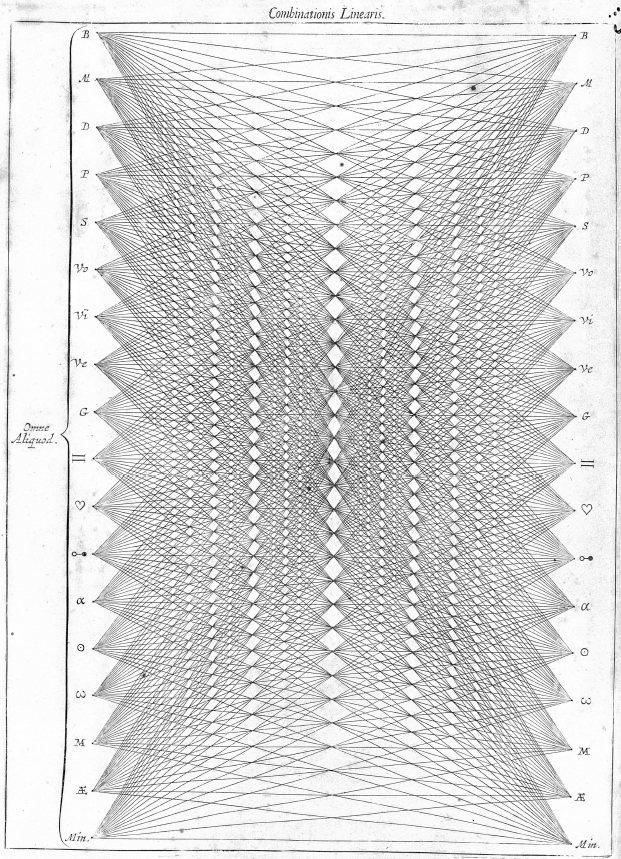
\includegraphics[scale=0.4]{k18x18.png} \begin{minipage}[b]{5cm}
 	$K_{18,18}$\newline A. Kircher (1669) \newline {\it Ars Magna Sciendi Sive Combinatoria}\end{minipage}
\end{center}

\end{frame}




\begin{frame}{Podstawowe grafy proste}
	\begin{block}{Inne}
		\begin{itemize}
			\item {\bf Graf dwudzielny} - graf w którym zbiór wierzchołków można podzielić na dwa rozłączne podzbiory $V_1,V_2$ takie, że
			$$E(G)\textcolor{red}{\subset}\big\{\{i,j\}:\,i\in V_1,\,j\in V_2\big\}.$$
			\item {\bf Drzewo} - graf spójny nie zawierający cykli.
			\item {\bf Las} - graf nie zawierający cykli.
			\item {\bf Graf $r$-regularny} - graf w którym stopień każdego wierzchołka wynosi $r$.
		\end{itemize}
	\end{block}

\begin{block}{Definicja}
Jeżeli $\deg v=1$ dla pewnego wierzchoła $v\in V(G)$, to $v$ nazywamy {\bf liściem}.
\end{block}
		
\end{frame}


\begin{frame}

\begin{block}{Twierdzenie}
Graf $G$ jest dwudzielny wtedy i tylko wtedy, gdy  $G$ nie zawiera cyklu nieparzystej długości.
\end{block}

\begin{block}{Dowód. {\it (1/2)}}
($\Rightarrow$)
Jeżeli $G$ jest grafem dwudzielnym, to $V(G)=V_1\cup V_2$, gdzie $V_1\cap V_2=\emptyset$. Niech $(v_1,v_2,\ldots,v_l)$ będzie cyklem długości $l$. 

\begin{minipage}{.38\textwidth}
Załóżmy (bez straty ogólności), że $v_1\in V_1$. Wtedy 
\begin{itemize}
\item $v_2\in V_2$,
\item $v_3\in V_1$,
\item $v_4\in V_2$,
\item $\ldots$,
\item $v_l\in V_2$.
\end{itemize}
Ogólnie $v_i\in V_1$ wtedy i tylko wtedy, gdy $i$ jest liczbą nieparzystą. Zatem $l$ jest liczbą parzystą.
\end{minipage}\hfill\begin{minipage}{.58\textwidth}
\begin{center}

\end{center}
\end{minipage}
\end{block}
\end{frame}


\begin{frame}

\begin{block}{Dowód. {\it (2/2)}}

($\Leftarrow$)

Zakładamy, że $G$ nie zawiera cyklu nieparzystej długości. 

\medskip

Graf $G$ jest dwudzielny wtedy i tylko wtedy, gdy każda jego składowa jest grafem dwudzielnym, więc możemy założyć, że $G$ jest spójny.

\medskip

Niech $x\in V(G)$ i niech $V_1$ będzie zbiorem wierzchołków, których odległość od $x$ jest nieparzysta i niech $V_2=V\backslash V_1$. Nie ma krawędzi łączących dwa wierzchołki ze zbioru $V_i$, bo gdyby taka krawędź istniała, to $G$ zawierałby cykl nieparzystej długości. Zatem $G$ jest dwudzielny.

\vfill\qed
\end{block}


\end{frame}


\end{document}